\chapter{实验结果}
\label{chap:results}

本章的实验在Linux系统上运行,CPU为i7-2620M($2.7\mbox{GHz}\times 4$),内存大小
为8GB。程序的核心代码基于C++及OpenCV实现。界面采用Qt编写。

在进行动作放大时,主要使用基于线性的欧拉影像动作放大方法,因此,本章的结果只和全
局的线性动作放大方法的结果进行对比。实验四将给出一个结合了本文的算法和基于相位的
方法的处理结果。

图\ref{fig:all-videos}罗列了本章所有实验案例的代表帧。

\begin{figure}[htbp]
  \centering
  \subfloat[实验一]{
    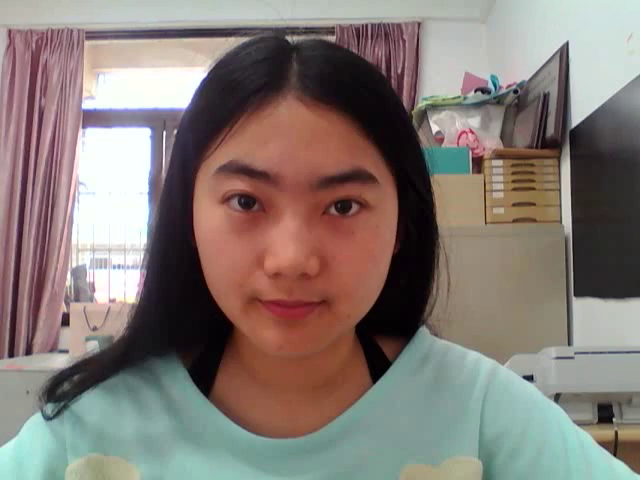
\includegraphics[height=4cm]{video1.png}
  }\qquad
  \subfloat[实验二]{
    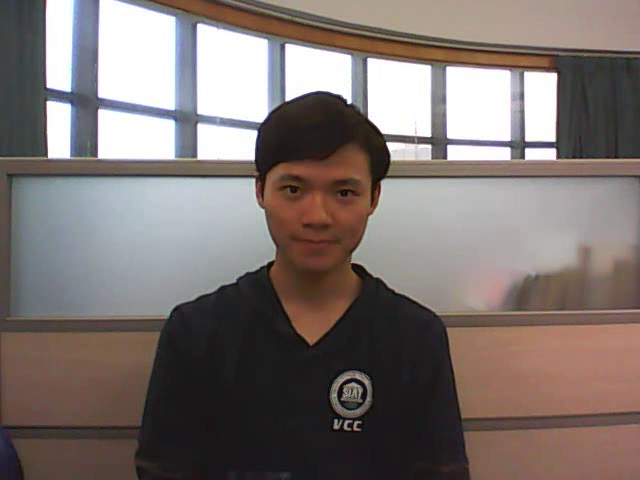
\includegraphics[height=4cm]{video2.png}
  }\\
  \subfloat[实验三]{
    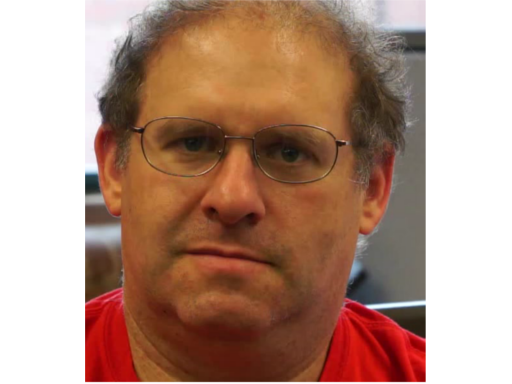
\includegraphics[height=4cm]{video3.png}
  }\qquad
  \subfloat[实验四]{
    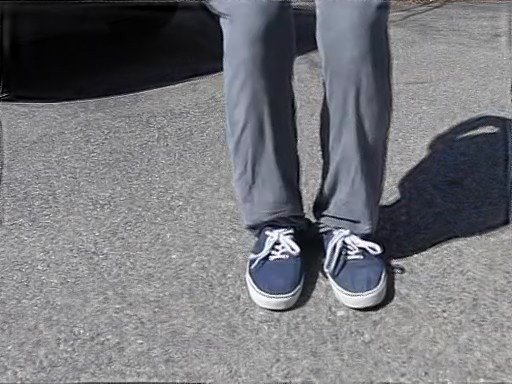
\includegraphics[height=4cm]{video4.png}
  }
  \caption{本章所有实验数据的代表帧}
  \label{fig:all-videos}
\end{figure}

\section{实验一}
\label{sec:exam1}

实验一的视频案例使用普通网路摄像头拍摄。在拍摄过程中,该实验对象被要求讲一段话。在讲
话时,她的头部有轻微摇动。

表\ref{tab:exam1-data}给出了相关实验参数。其中,$\alpha$是放大倍数,
$w_l$和$w_h$是带通滤波的下界和上界,$f_s$是视频的帧率。

\begin{table}[htbp]
  \centering
  \caption{实验一的相关实验参数}
  \label{tab:exam1-data}
  \begin{tabular}[c]{crrrr}
    \toprule[1.5pt]
    放大类型 & $\alpha$ & $w_l$(Hz) & $w_h$ (Hz) & $f_s$(Hz)\\
    \midrule
    动作变化 & 20 & 0.1 & 0.5 & 25 \\
    颜色变化 & 100 & 0.83 & 1 & 25 \\
    \bottomrule[1.5pt]
  \end{tabular}
\end{table}

对视频分别进行全局的线性欧拉影像动作放大和本文所提出的前景约束的欧拉影像动作放大,
结果如图\ref{fig:exam1-result}所示。其中,图\ref{fig:exam1-reference}最左侧子图的
绿框和黄线分别代表了实验所选择的感兴趣区域和XT切片所选取的位置。由XT切片可以看出,
全局的线性动作变化放大算法会连同背景区域一起放大,对放大结果造成一定影响。

\begin{figure}[htbp]
  \centering
  \subfloat[输入视频及XT切片]{
    \label{fig:exam1-reference}
    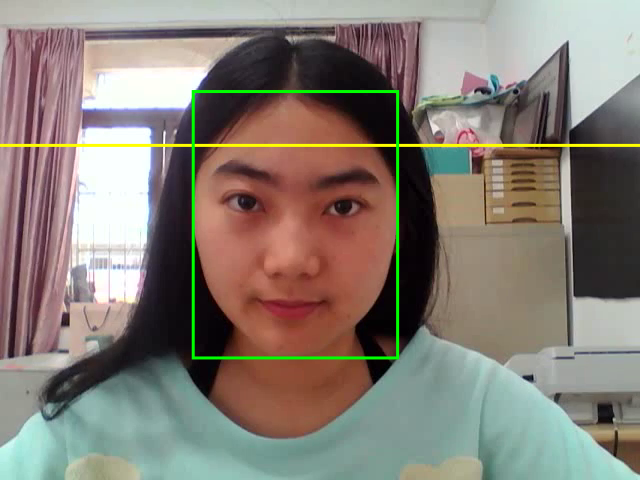
\includegraphics[width=.3\textwidth]{video1-0.png}~
    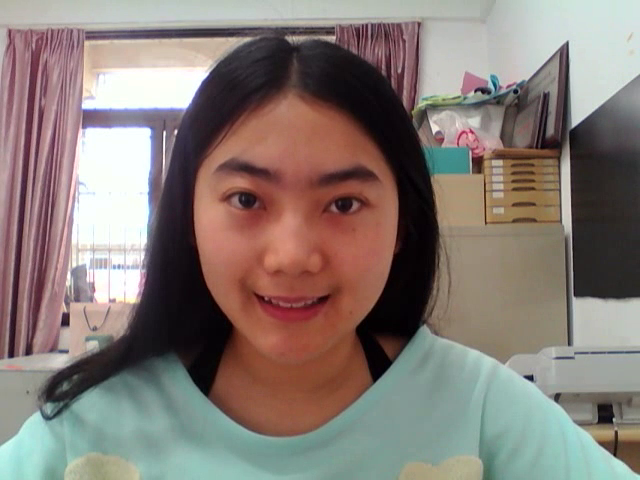
\includegraphics[width=.3\textwidth]{video1-1.png}\qquad
    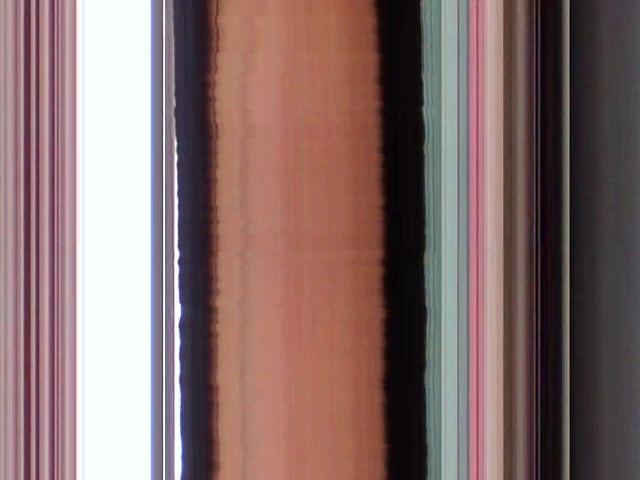
\includegraphics[width=.3\textwidth]{video1-XT.png}
  }\\
  \subfloat[全局的线性动作变化放大结果及XT切片]{
    
\includegraphics[width=.3\textwidth]{video1-motion-linear-0.png}~
    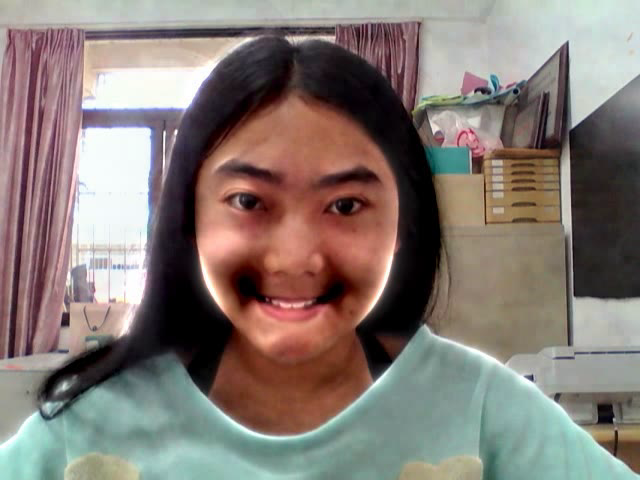
\includegraphics[width=.3\textwidth]{video1-motion-linear-1.png}\qquad
    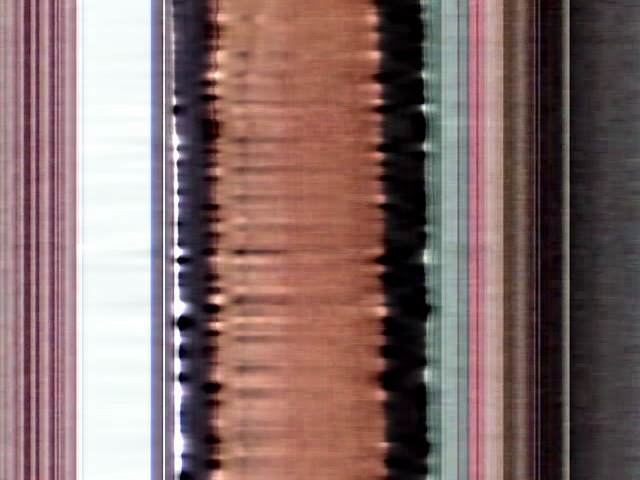
\includegraphics[width=.3\textwidth]{video1-motion-linear-XT.png}
  }\\
  \subfloat[前景约束的动作变化放大结果及XT切片]{
    
\includegraphics[width=.3\textwidth]{video1-motion-fc-0.png}~
    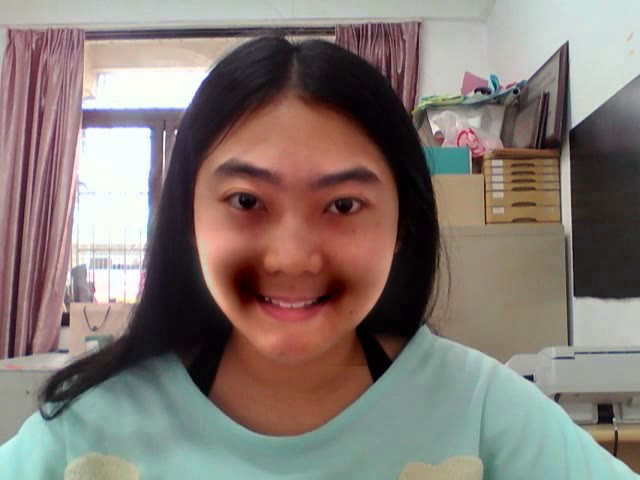
\includegraphics[width=.3\textwidth]{video1-motion-fc-1.png}\qquad
    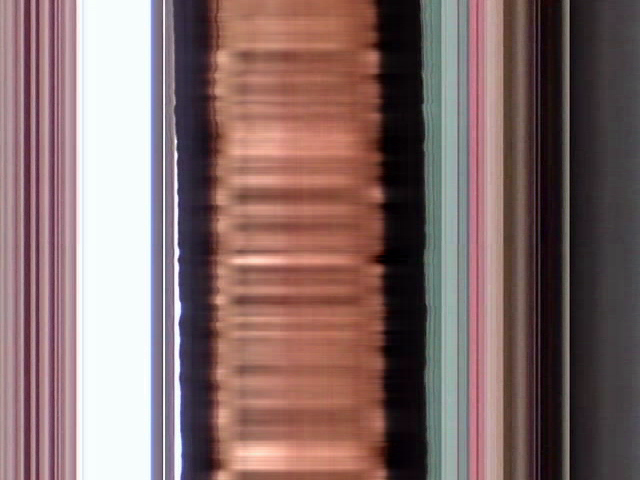
\includegraphics[width=.3\textwidth]{video1-motion-fc-XT.png}
  }\\
  \subfloat[全局的线性颜色变化放大结果及XT切片]{
    
\includegraphics[width=.3\textwidth]{video1-color-linear-0.png}~
    
\includegraphics[width=.3\textwidth]{video1-color-linear-1.png}\qquad
    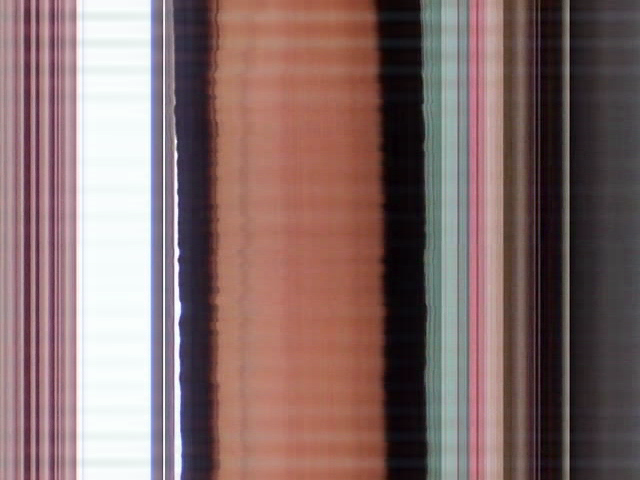
\includegraphics[width=.3\textwidth]{video1-color-linear-XT.png}
  }\\
  \subfloat[前景约束的颜色变化放大结果及XT切片]{
    
\includegraphics[width=.3\textwidth]{video1-color-fc-0.png}~
    
\includegraphics[width=.3\textwidth]{video1-color-fc-1.png}\qquad
    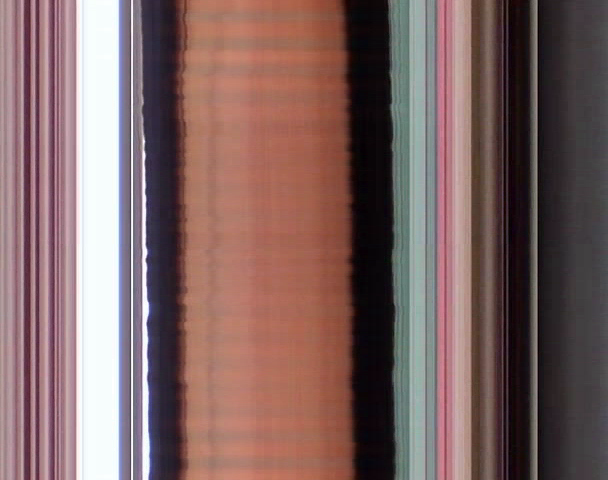
\includegraphics[width=.3\textwidth]{video1-color-fc-XT.png}
  }
  \caption{实验一的放大结果}
  \label{fig:exam1-result}
\end{figure}

实验一的算法执行速度如表\ref{tab:time1}所示。由表可知,本文的算法主要耗时在于前景
分割模块。当不使用GrabCut算法进行前景分割时,算法的速度比全局线性的方法快了接
近2.5倍。这是由于欧拉影像放大是逐像素进行的,而目标区域比原图区域的范围小,因此可
以达到更快的处理速度。然而,如果对放大效果有更高的要求,使用GrabCut算法则可以很好
的去除边界。在本文所提供的动作放大系统中,前景分割是一个可选项,以方便用户在速
度和效果间做权衡。

\begin{table}[htbp]
  \centering
  \caption{实验一的程序执行速度(fps)}
  \label{tab:time1}
  \begin{tabular}[c]{rrr}
    \toprule[1.5pt]
    线性的方法 & 不分割前景 & 分割前景 \\
    \midrule
    14.47 & 36.36 & 2.20 \\
    \bottomrule[1.5pt]
  \end{tabular}
\end{table}

\section{实验二}
\label{sec:man-moving}

实验二的视频案例使用普通网路摄像头拍摄。在拍摄过程中,该实验对象被要求随意移动身体,
使身体出现较大幅度的动作。

表\ref{tab:exam2-data}给出了相关实验参数。

\begin{table}[htbp]
  \centering
  \caption{实验二的相关实验参数}
  \label{tab:exam2-data}
  \begin{tabular}[c]{crrrr}
    \toprule[1.5pt]
    放大类型 & $\alpha$ & $w_l$(Hz) & $w_h$ (Hz) & $f_s$(Hz)\\
    \midrule
    动作变化 & 10 & 0.05 & 0.4 & 20 \\
    颜色变化 & 150 & 0.83 & 1 & 20 \\
    \bottomrule[1.5pt]
  \end{tabular}
\end{table}

图\ref{fig:exam2-result}给出了两种方法的实验结果对比。
图\ref{fig:exam2-reference}最左侧子图的绿框和黄线分别代表了实验所选择的感兴趣区域
和XT切片所选取的位置。由于该实验对象的运动幅度较大,此时直接进行全局的动作放大会
出现明显的“鬼影”问题,且颜色变化的放大结果也受到了该实验对象身体的移动的影响,
导致无法正确地放大其脸部颜色的变化。而前景约束的动作放大则可以在避免对身体移动的
放大的同时有效地放大脸部的动作变化和颜色变化。

\begin{figure}[htbp]
  \centering
  \subfloat[输入视频及XT切片]{
    \label{fig:exam2-reference}
    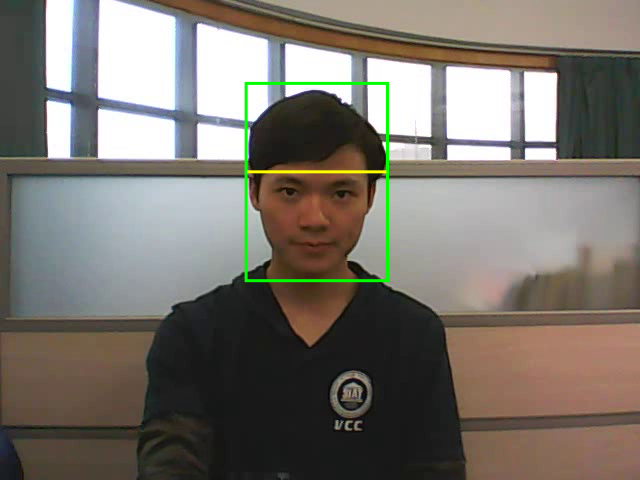
\includegraphics[height=3.3cm]{video2-0.png}~
    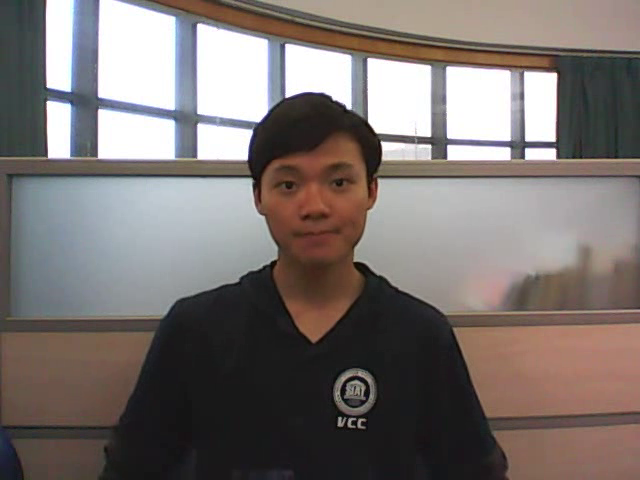
\includegraphics[height=3.3cm]{video2-1.png}\qquad
    \scalebox{2}[1]{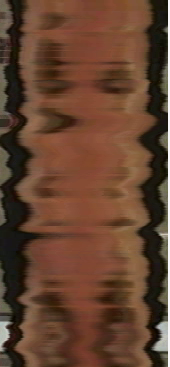
\includegraphics[height=3.3cm]{video2-XT.png}}
  }\\
  \subfloat[全局的线性动作变化放大结果及XT切片]{
    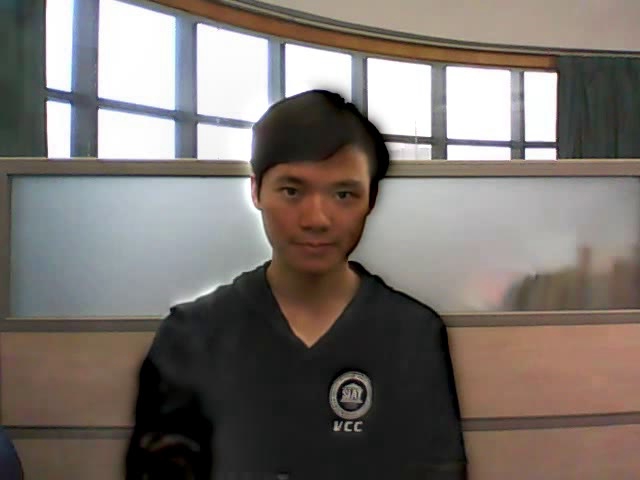
\includegraphics[height=3.3cm]{video2-motion-linear-0.png}~
    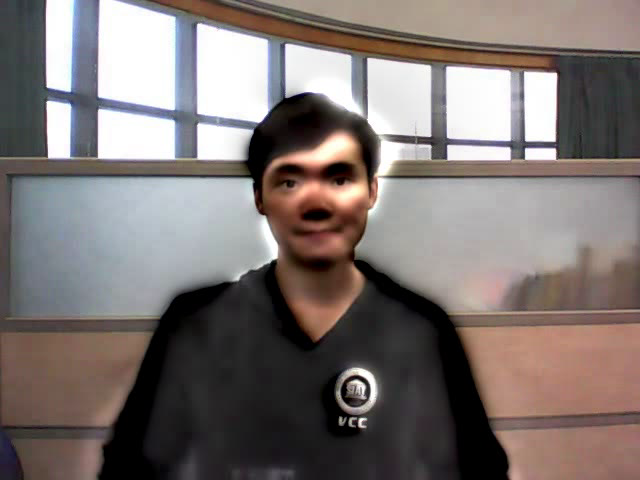
\includegraphics[height=3.3cm]{video2-motion-linear-1.png}\qquad
    \scalebox{2}[1]{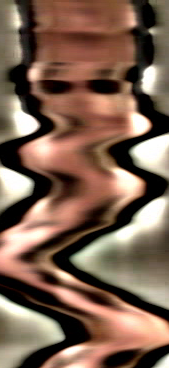
\includegraphics[height=3.3cm]{video2-motion-linear-XT.png}}
  }\\
  \subfloat[前景约束的动作变化放大结果及XT切片]{
    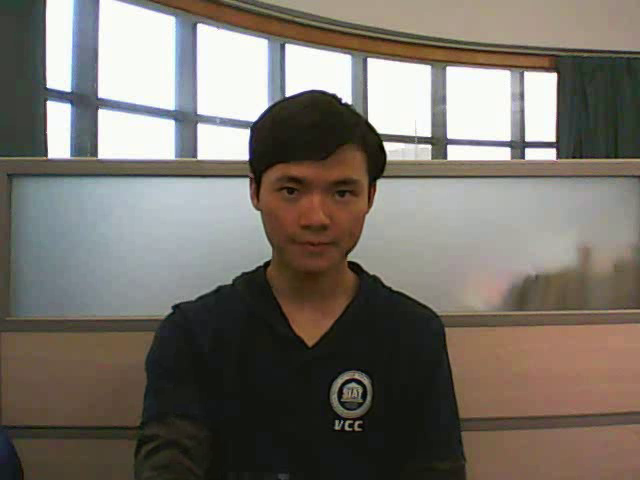
\includegraphics[height=3.3cm]{video2-motion-fc-0.png}~
    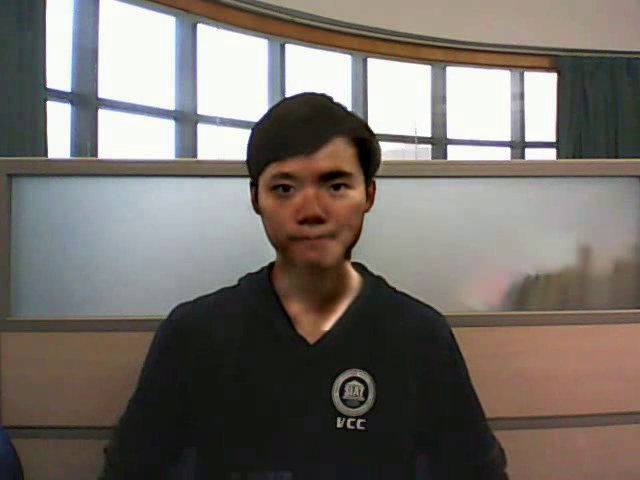
\includegraphics[height=3.3cm]{video2-motion-fc-1.png}\qquad
    \scalebox{2}[1]{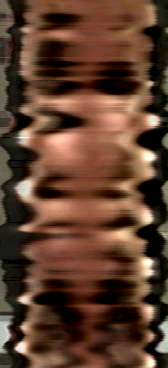
\includegraphics[height=3.3cm]{video2-motion-fc-XT.png}}
  }\\
  \subfloat[全局的线性颜色变化放大结果及XT切片]{
    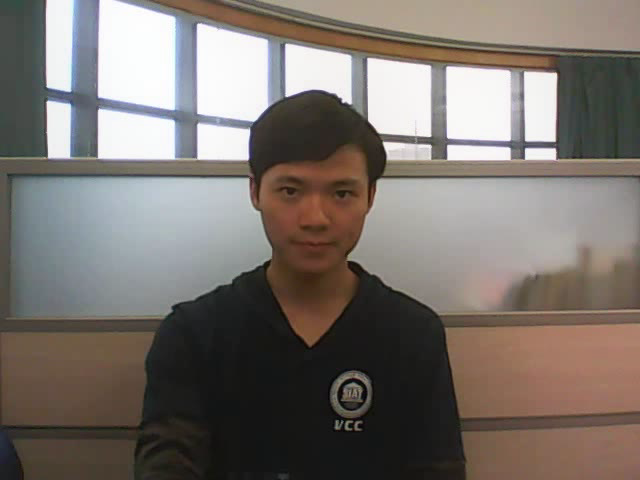
\includegraphics[height=3.3cm]{video2-color-linear-0.png}~
    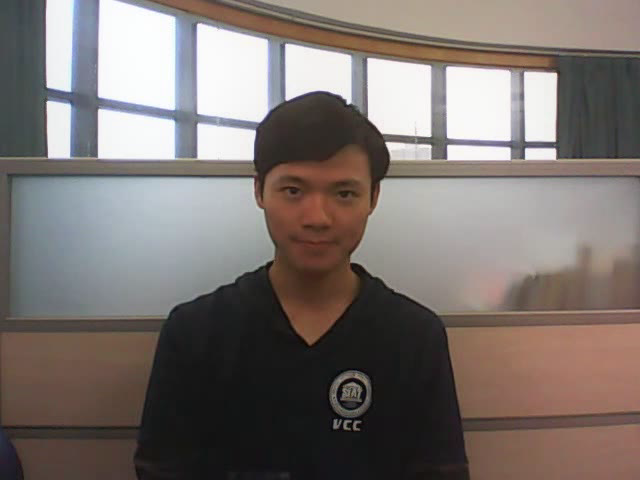
\includegraphics[height=3.3cm]{video2-color-linear-1.png}\qquad
    \scalebox{2}[1]{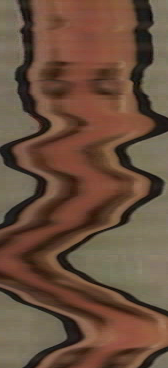
\includegraphics[height=3.3cm]{video2-color-linear-XT.png}}
  }\\
  \subfloat[前景约束的颜色变化放大结果及XT切片]{
    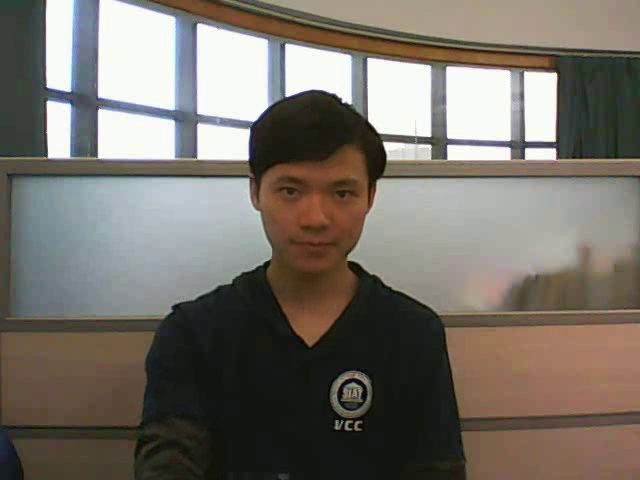
\includegraphics[height=3.3cm]{video2-color-fc-0.png}~
    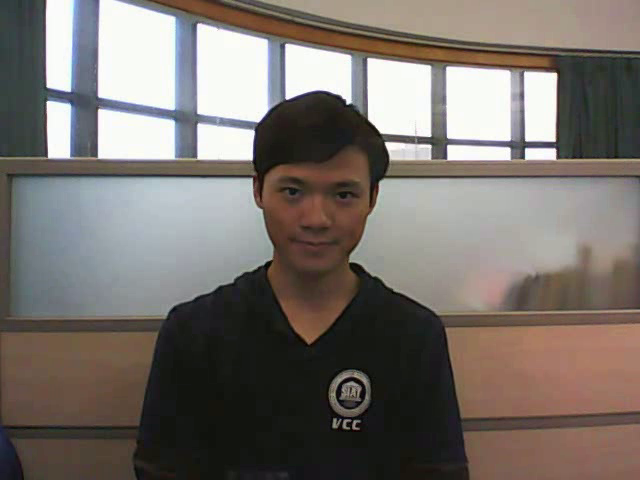
\includegraphics[height=3.3cm]{video2-color-fc-1.png}\qquad
    \scalebox{2}[1]{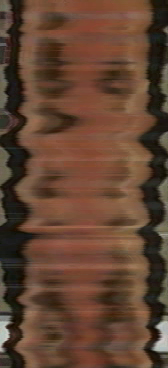
\includegraphics[height=3.3cm]{video2-color-fc-XT.png}}
  }
  \caption{实验二的放大结果}
  \label{fig:exam2-result}
\end{figure}

实验二的算法执行速度如表 \ref{tab:time2} 所示。

\begin{table}[htbp]
  \centering
  \caption{实验二的程序执行速度(fps)}
  \label{tab:time2}
  \begin{tabular}[c]{rrr}
    \toprule[1.5pt]
    线性的方法 & 不分割前景 & 分割前景 \\
    \midrule
    15.44 & 48.78 & 2.68 \\
    \bottomrule[1.5pt]
  \end{tabular}
\end{table}


\section{实验三}
\label{sec:exam-face}

实验三的视频案例出自文献\cite{wu2012eulerian}中的face案例。表\ref{tab:exam3-data}给出了相关实验参数。

\begin{table}[htbp]
  \centering
  \caption{实验三的相关实验参数}
  \label{tab:exam3-data}
  \begin{tabular}[c]{crrrr}
    \toprule[1.5pt]
    放大类型 & $\alpha$ & $w_l$(Hz) & $w_h$ (Hz) & $f_s$(Hz)\\
    \midrule
    动作变化 & 40 & 0.05 & 0.4 & 20 \\
    颜色变化 & 100 & 0.83 & 1 & 20 \\
    \bottomrule[1.5pt]
  \end{tabular}
\end{table}

图\ref{fig:exam3-result}给出了两种方法的实验结果对比。
图\ref{fig:exam3-reference}最左侧子图的绿框和黄线分别代表了实验所选择的感兴趣区域
和YT切片所选取的位置。和实验一类似,使用本文提出的前景约束的方法可以避免对背景区
域的放大。实验三的结果进一步说明了即使场景中不存在明显的动作,使用本文的算法也可
以得到比全局的放大方法更好的实验结果。

\begin{figure}[htbp]
  \centering
  \subfloat[输入视频及YT切片]{
    \label{fig:exam3-reference}
    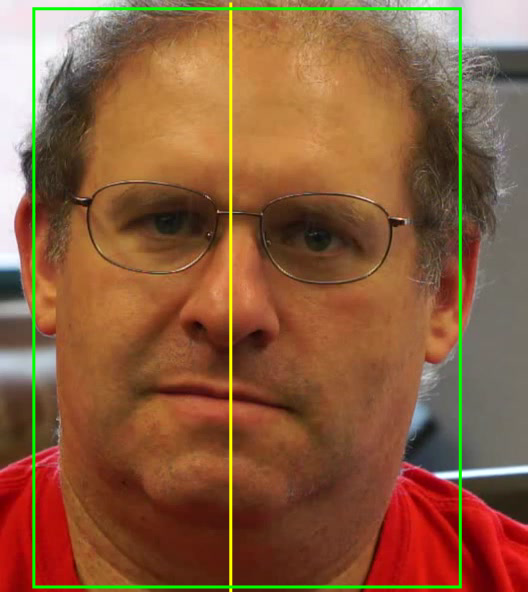
\includegraphics[height=3.3cm]{video3-0.png}~
    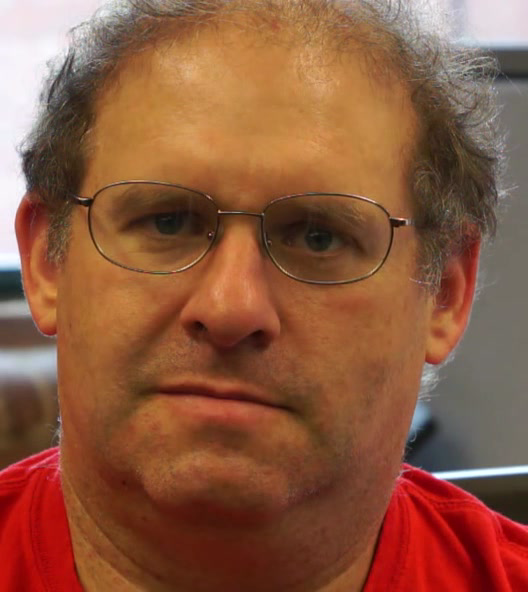
\includegraphics[height=3.3cm]{video3-1.png}\qquad
    \scalebox{2}[1]{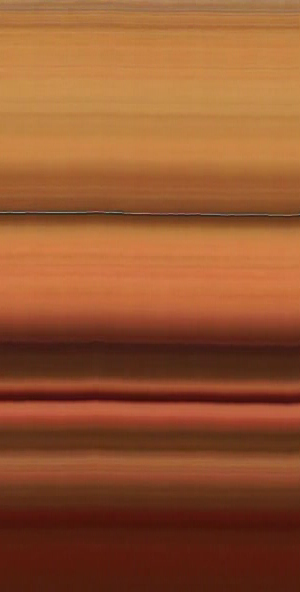
\includegraphics[height=3.3cm]{video3-YT.png}}
  }\\
  \subfloat[全局的线性动作变化放大结果及YT切片]{
    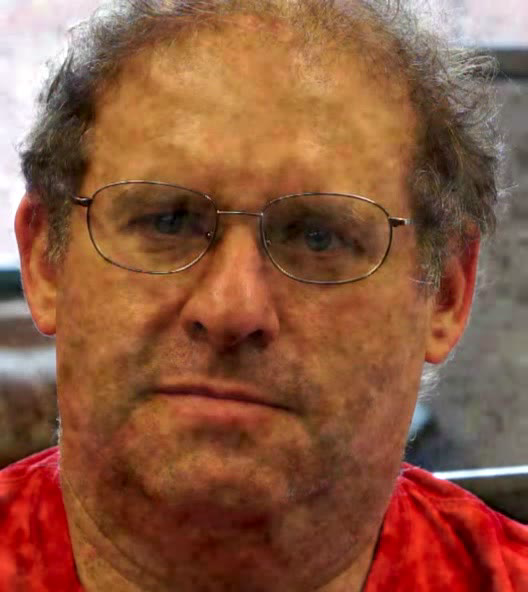
\includegraphics[height=3.3cm]{video3-motion-linear-0.png}~
    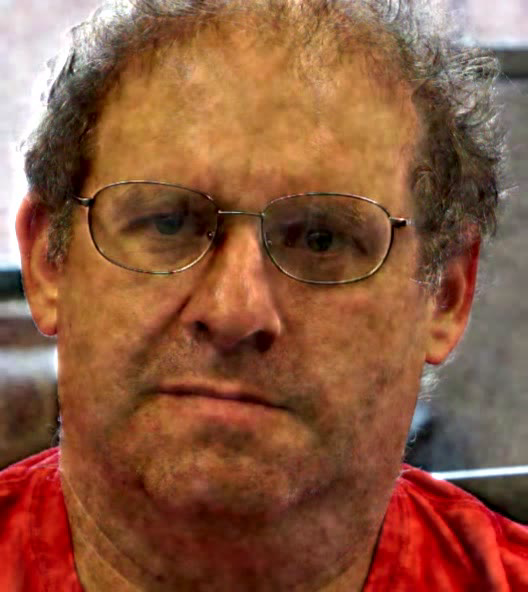
\includegraphics[height=3.3cm]{video3-motion-linear-1.png}\qquad
    \scalebox{2}[1]{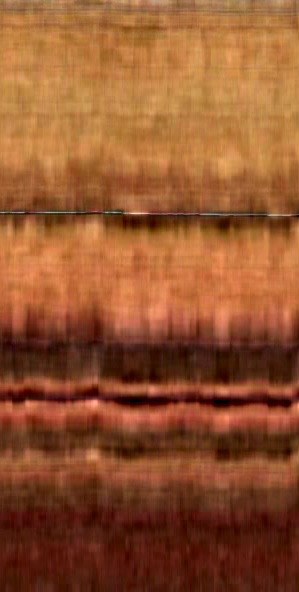
\includegraphics[height=3.3cm]{video3-motion-linear-YT.png}}
  }\\
  \subfloat[前景约束的动作变化放大结果及YT切片]{
    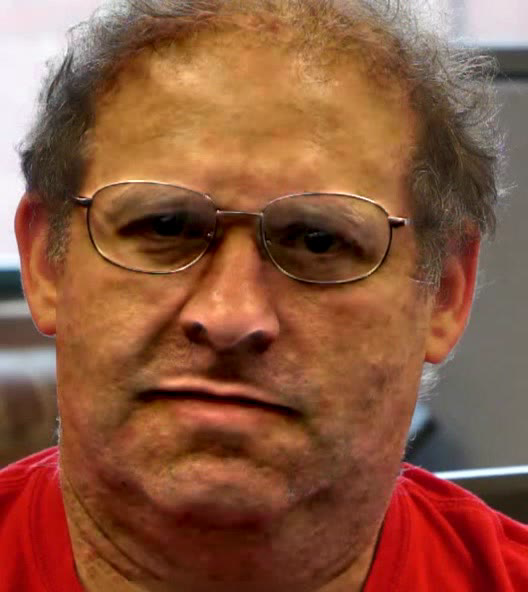
\includegraphics[height=3.3cm]{video3-motion-fc-0.png}~
    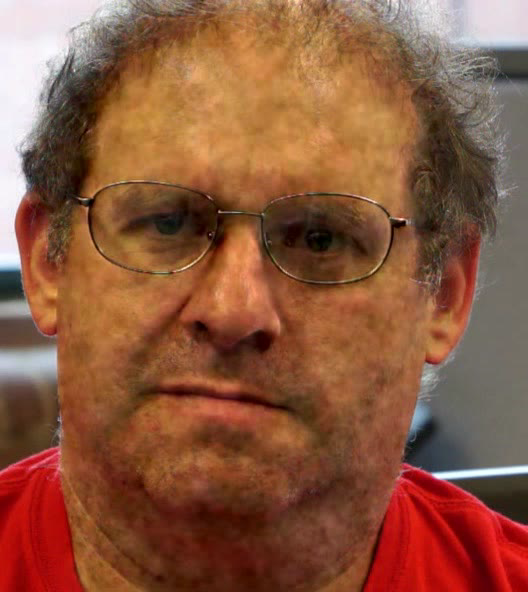
\includegraphics[height=3.3cm]{video3-motion-fc-1.png}\qquad
    \scalebox{2}[1]{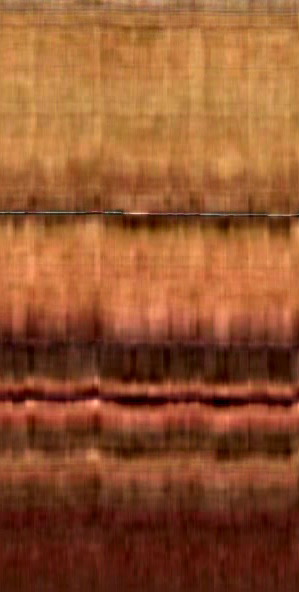
\includegraphics[height=3.3cm]{video3-motion-fc-YT.png}}
  }\\
  \subfloat[全局的线性颜色变化放大结果及YT切片]{
    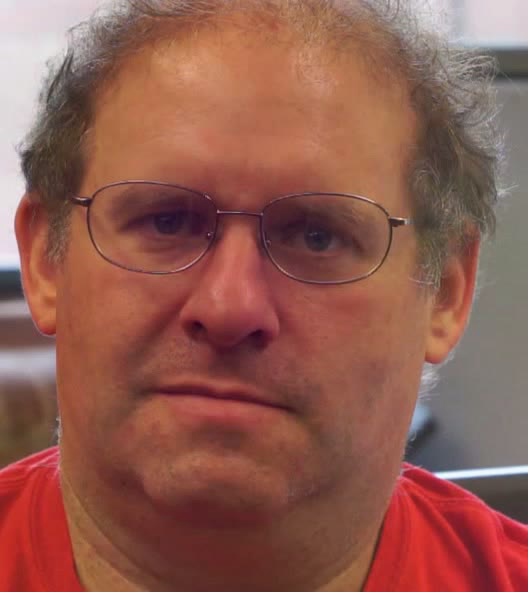
\includegraphics[height=3.3cm]{video3-color-linear-0.png}~
    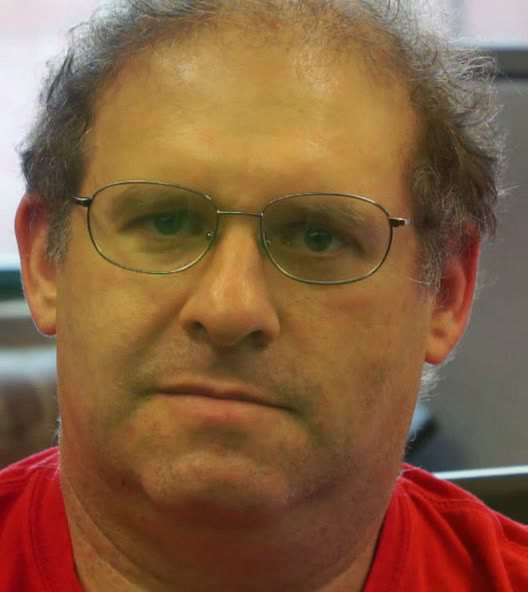
\includegraphics[height=3.3cm]{video3-color-linear-1.png}\qquad
    \scalebox{2}[1]{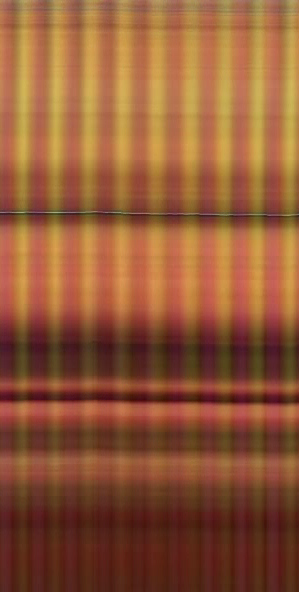
\includegraphics[height=3.3cm]{video3-color-linear-YT.png}}
  }\\
  \subfloat[前景约束的颜色变化放大结果及YT切片]{
    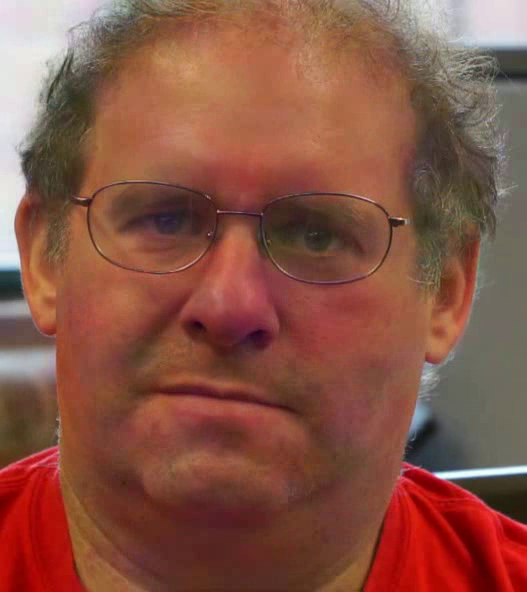
\includegraphics[height=3.3cm]{video3-color-fc-0.png}~
    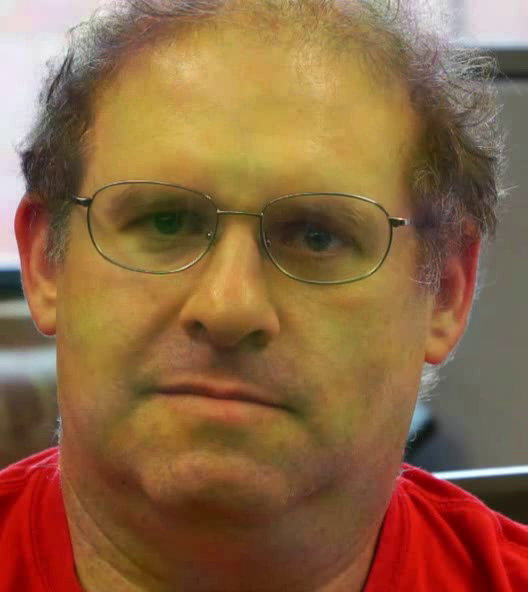
\includegraphics[height=3.3cm]{video3-color-fc-1.png}\qquad
    \scalebox{2}[1]{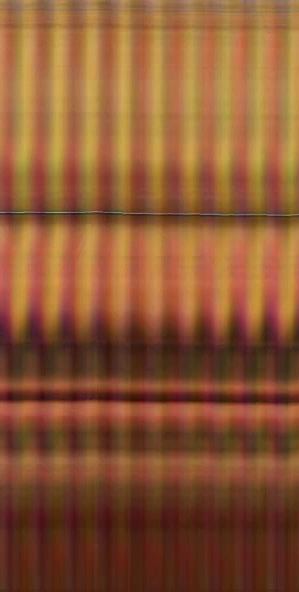
\includegraphics[height=3.3cm]{video3-color-fc-YT.png}}
  }
  \caption{实验三的放大结果}
  \label{fig:exam3-result}
\end{figure}

实验三的算法执行速度如表 \ref{tab:time3} 所示。

\begin{table}[htbp]
  \centering
  \caption{实验二的程序执行速度(fps)}
  \label{tab:time3}
  \begin{tabular}[c]{rrr}
    \toprule[1.5pt]
    线性的方法 & 不分割前景 & 分割前景 \\
    \midrule
    13.78 & 17.45 & 1.45 \\
    \bottomrule[1.5pt]
  \end{tabular}
\end{table}

\section{实验四}
\label{sec:exam-stomp}

本实验将演示结合了基于相位的方法和前景约束的方法同时放大感兴趣区域和其他区域的方
法。

实验四的视频案例出自文献\cite{Wadhwa2013PhaseBased}中的stomp案例。先对该视频进行
基于相位的放大,在进行动作放大前,先通过相位变化判断出哪些部分的动作幅度较大,之
后在放大过程中忽略这些部分(通过将放大倍数设为0)。经过放大后,可以明显的观察出双脚着
地后地面的震动。

之后,再从基于相位的动作放大过程中所忽略的部分中标出感兴趣的区域,对该区域再进行
一次前景约束的放大。作为示例,这里选择放大膝盖部分的动作。同时为了加快速度,取消
了前景分割。在使用本文的算法进行第二次动作放大时,处理速度达49帧/秒。

图\ref{fig:exam4-result}给出了两步放大的结果。其中,
图\ref{fig:exam4-reference-1}和图\ref{fig:exam4-reference-2}最左侧子图的黄线都代
表了该图的YT切片所选取的位置。图\ref{fig:exam4-reference-2}最左侧子图的绿线代表
了所选择的感兴趣区域。

\begin{figure}[htbp]
  \centering
  \subfloat[输入视频及YT切片]{
    \label{fig:exam4-reference-1}
    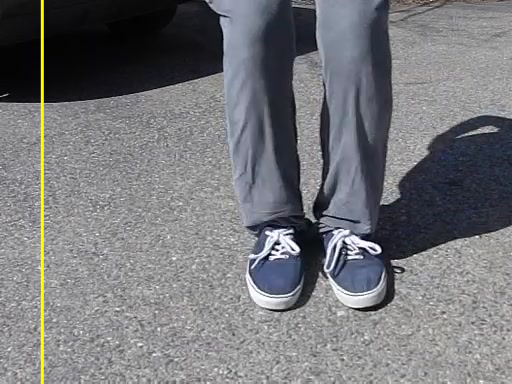
\includegraphics[height=3.3cm]{video4-0.png}~
    \includegraphics[height=3.3cm]{video4-1.png}\qquad
    \scalebox{2}[1]{\includegraphics[height=3.3cm]{video4-YT.png}}
  }\\
  \subfloat[基于相位的动作放大结果及YT切片]{
    \includegraphics[height=3.3cm]{video4-phase-0.png}~
    \includegraphics[height=3.3cm]{video4-phase-1.png}\qquad
    \scalebox{2}[1]{\includegraphics[height=3.3cm]{video4-phase-YT.png}}
  }\\
  \subfloat[前景约束的动作变化放大结果及放大前后的YT切片]{
    \label{fig:exam4-reference-2}
    \includegraphics[height=3.3cm]{video4-fc-0.png}~
    \includegraphics[height=3.3cm]{video4-fc-1.png}\qquad
    \includegraphics[height=3.3cm]{video4-fc-YT-before.png}\qquad
    \includegraphics[height=3.3cm]{video4-fc-YT-after.png}
  }\\
  \caption{实验四的放大结果}
  \label{fig:exam4-result}
\end{figure}

从图\ref{fig:exam4-result}中可知,经过两步放大后,地面的震动和膝盖部位的光线变化
得到了增强。因此,通过使用全局的欧拉影像放大方法和本文所提出的前景约束的方法相结
合的方法,既可以放大场景中存在大幅度动作的物体中的细微动作,也可以放大场景中的其
他区域,而且可以有效的防止出现“鬼影”问题。

%%% Local Variables: 
%%% mode: latex
%%% TeX-master: "../thesis"
%%% End: 
